\chapter{Performancemessungen}

\section{Tests von Audio�bertragung}
\subsection{Bandbreite}
-- Verbrauch der Bandbreite mit zunehmender Nutzerzahl beim "`Full mesh"'
-- Verbrauch der Bandbreite mit zunehmender Nutzerzahl beim "`Partial mesh"' 
-- Ballungszentren f�hren zu fullmesh --> zeigen

--> M�sste zeigen dass im Schnitt bei einer gleichm��igen Avatarverteilung die der Verbrauch geringer ist.
--> Messung mit Wireshark

\subsection{Bandbreite vs. Entfernung}
Um zu zeigen, dass das Verfahren auch tats�chlich Bandbreite einsparen kann, haben wir in einem Versuchsaufbau die Bandbreite in den verschiedenen Kommunikationszonen gemessen. Dabei ist klar ersichtlich dass durch ein Herausnehmen beider Teilnehmer aus der Konferenz somit kein Audio mehr �bertragen wird und der VAD die silence detection einschaltet.

\subsection{ohne Alles}

\begin{figure}[htbp]
	\centering
	\caption{Der Up- und Downstream}
		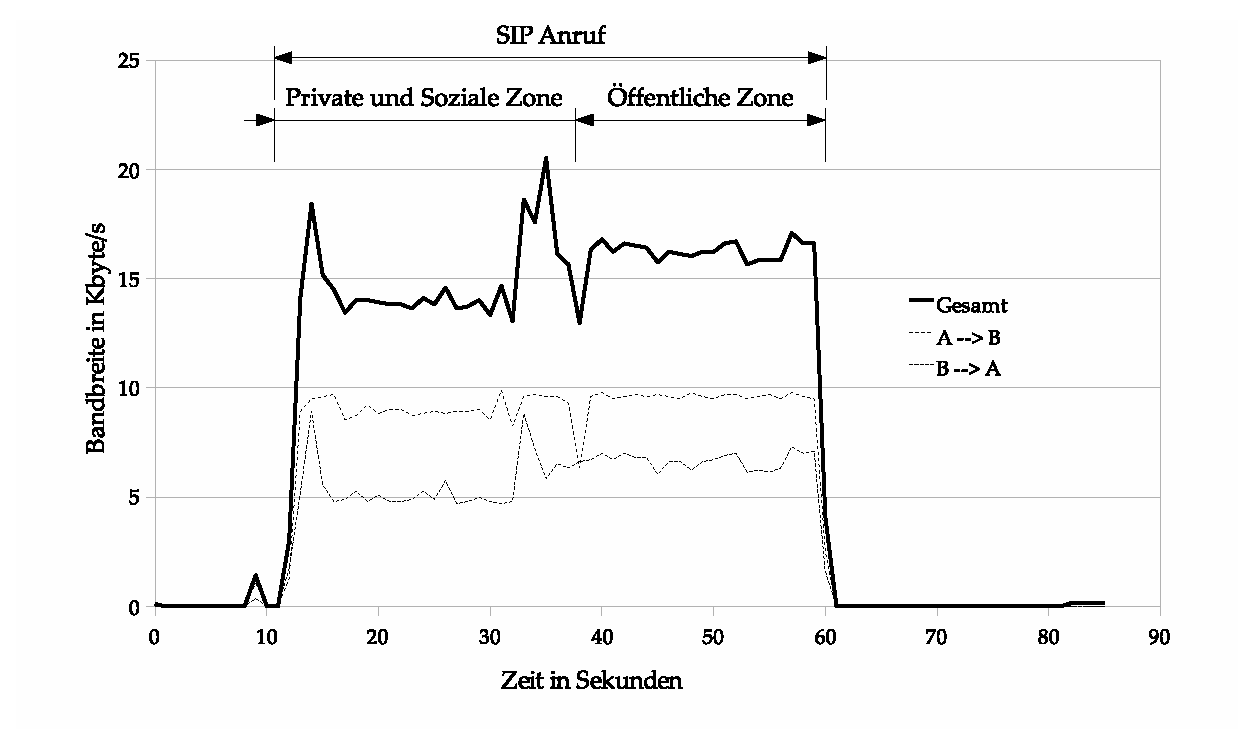
\includegraphics[width=1.00\textwidth]{grafiken/ohnevpn1.eps}
	\label{fig:NOVADrtpsip}
\end{figure}

\begin{figure}[htbp]
	\centering
	\caption{Gegen�berstellung der SIP und RTP}
		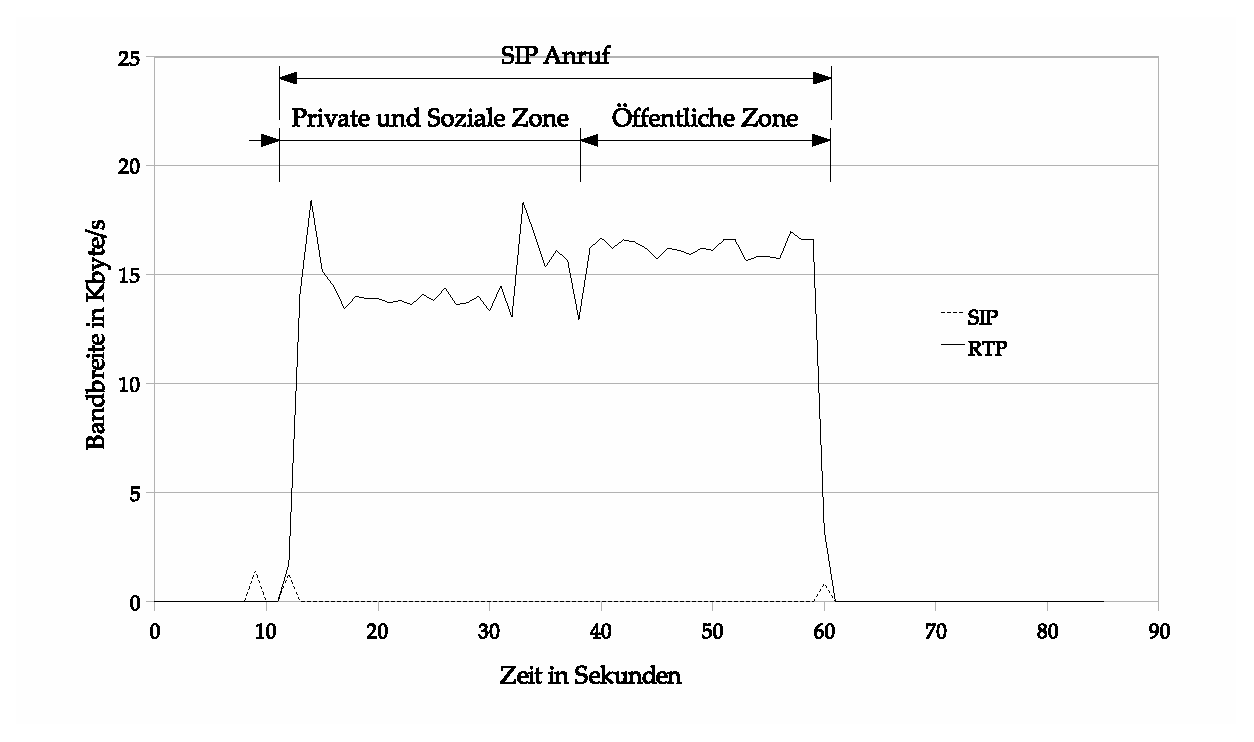
\includegraphics[width=1.00\textwidth]{grafiken/ohnevpn2.eps}
	\label{fig:NoVADupdown}
\end{figure}


\subsection{mit RTP manual Silence Supression}

\begin{figure}[htbp]
	\centering
	\caption{Der Up- und Downstream mit der VAD - Technik}
		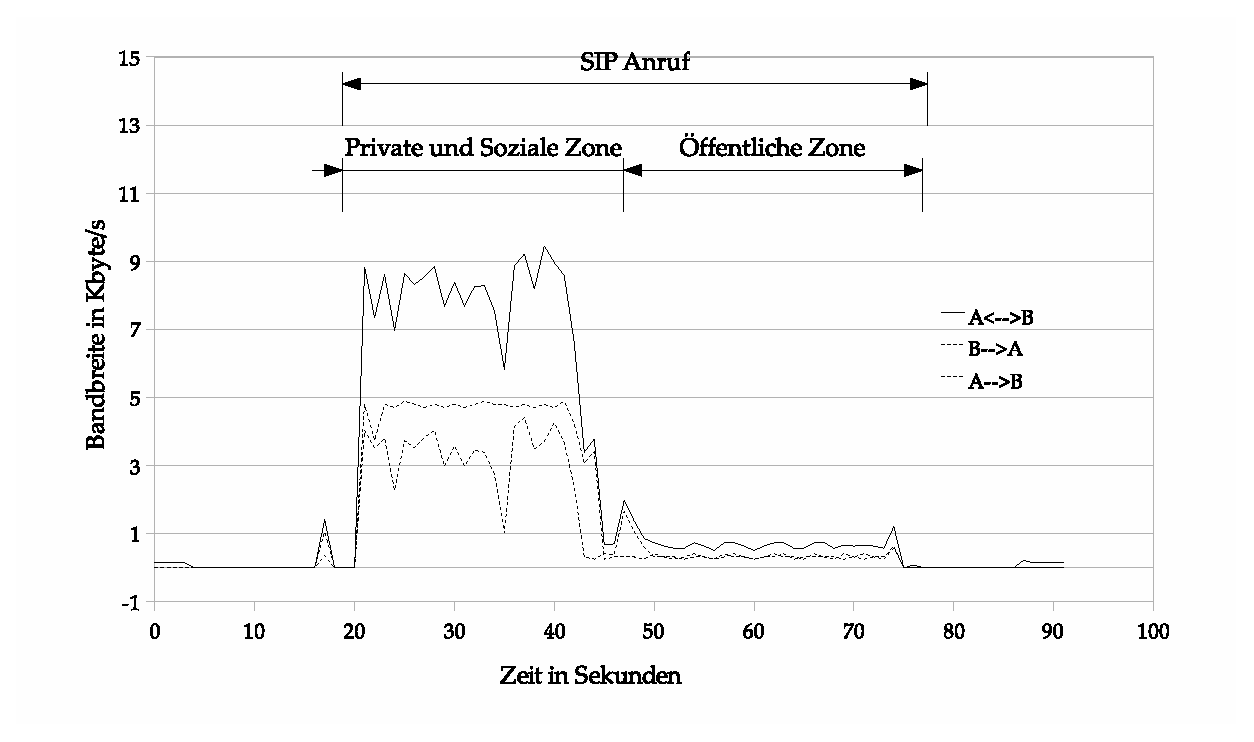
\includegraphics[width=1.00\textwidth]{grafiken/mitvadupdown.eps}
	\label{fig:NoVADupdown}
\end{figure}

\begin{figure}[htbp]
	\centering
		\caption{Gegen�berstellung der SIP und RTP Traffics mit der VAD - Technik}
		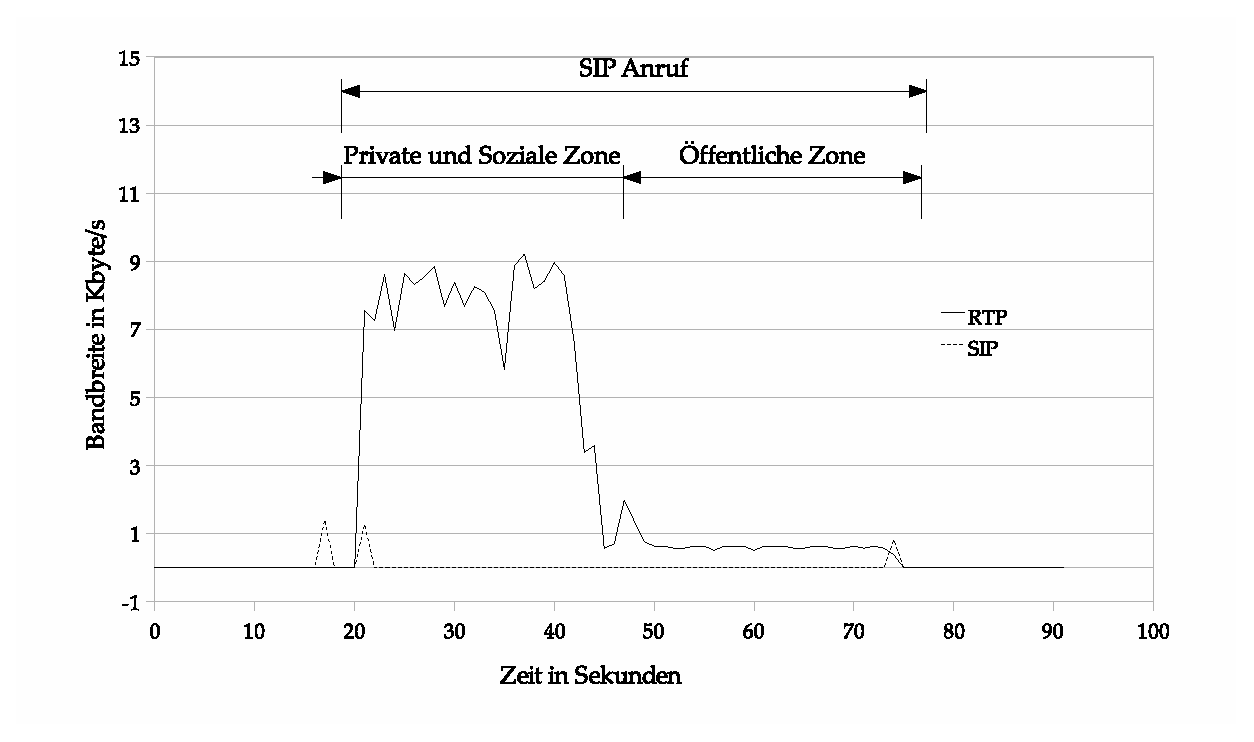
\includegraphics[width=1.00\textwidth]{grafiken/mitvadrtpsip.eps}
	\label{fig:NoVADupdown}
\end{figure}




\subsection{mit SIP HOLD}

\begin{figure}[htbp]
	\centering
	\caption{Der Up- und Downstream mit der SIP HOLD - Technik}
		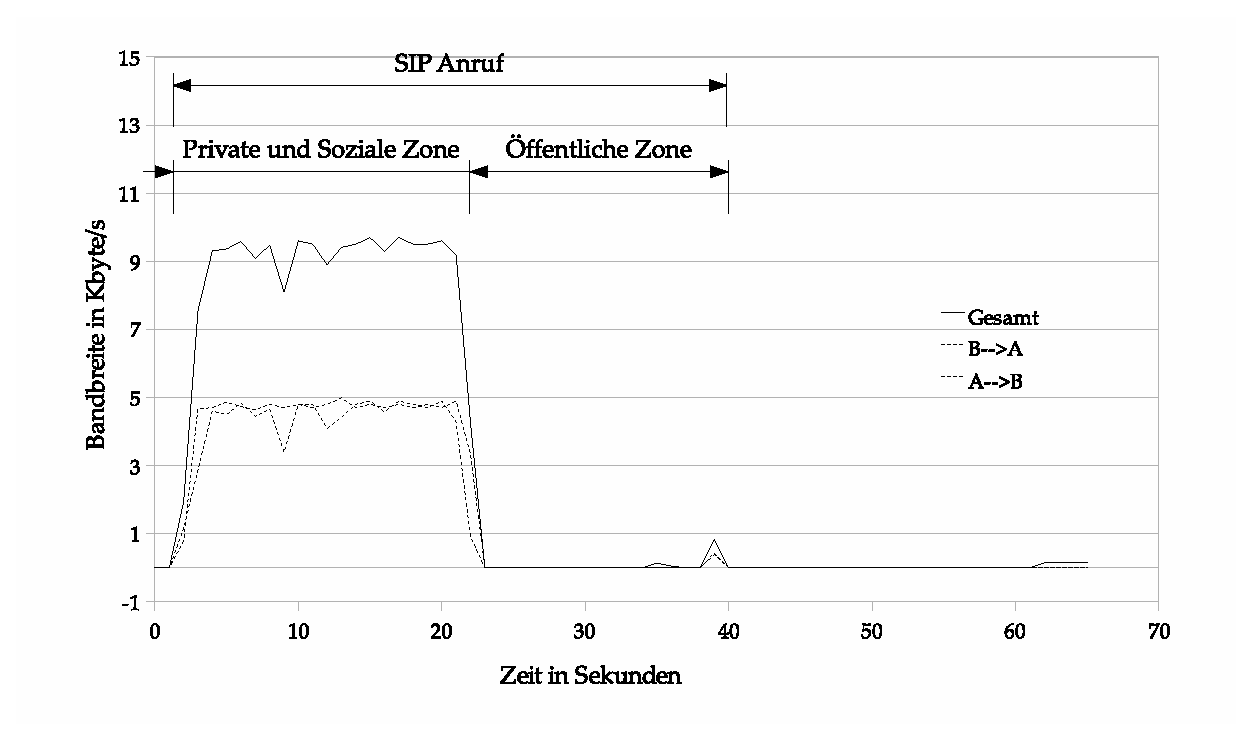
\includegraphics[width=1.00\textwidth]{grafiken/mitholdupanddown.eps}
	\label{fig:mitholdupanddown}
\end{figure}

\begin{figure}[htbp]
	\centering
	\caption{Gegen�berstellung des SIP und RTP Traffics mit der SIP HOLD - Technik}
		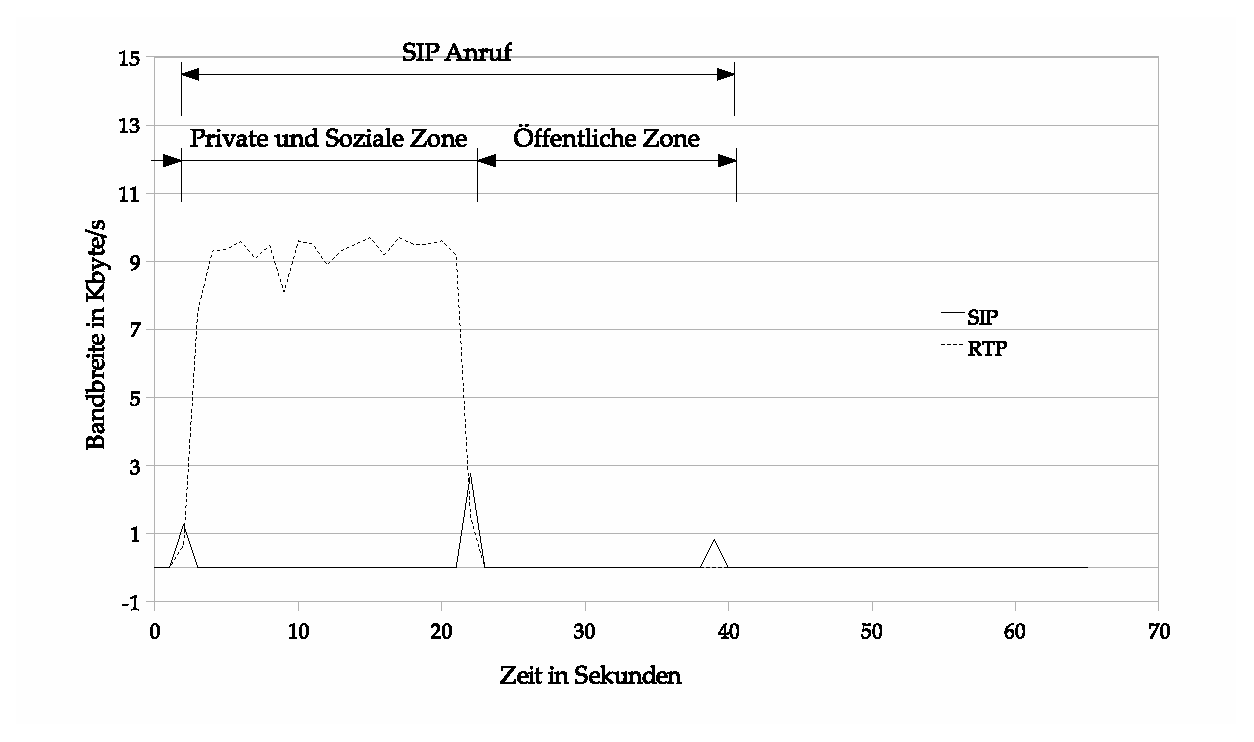
\includegraphics[width=1.00\textwidth]{grafiken/mithold1.eps}
	\label{fig:mithold1}
\end{figure}


-- Verbrauch der Bandbreite mit zunehmender Entfernung
--> M�sste zeigen dass beim "`silencen"' der RTP Session weniger Bandbreite verbraucht wird.
--> Messung mit Wireshark
-->DONE

\subsection{Mixing}
-- Verbrauch der CPU Last mit Zunehmender Nutzerzahl beim Full Mesh 
-- Verbrauch der CPU Last mit Zunehmender Nutzerzahl beim Partial Mesh
--> M�sste zeigen dass weniger Streams gemischt werden m�ssen und somit Last eingespart werden kann. ( Wie messe ich das?)
MESSUNG: einfach nur die conference bridge messen.

\subsection{Ende-zu-Ende Verz�gerung (Delay)}
-- delay �ber zeit bei mehreren verteilten stationen
\subsection{Verz�gerungsschwankung (Jitter)}
-- jitter �ber zeit bei mehreren verteilten stationen
\subsection{Paketverlust (Packet Loss)}
-- packetloss �ber zeit bei mehreren verteilten stationen

\section{Tests von SIP als Netzwerkschnitstelle}
-- RTT �ber die zeit bei konstanten benutzern vs. Resultat mit Multicast Sockets oder Skype.
